% !TeX root = ../main.tex

\chapter{Synthesis and Implementation}

The last step of this project is performed by Vivado. After the description and the testing phase have been completed, Vivado provided the synthesis and the implementation on FPGA board. The out-of-context mode has been set in the implementation phase due to the absence of physical board. In this chapter all the steps are analyzed, from the synthesis to the implementation.

\section{Synthesis}

\subsection{Warning messages}

Before illustrating the synthesis analysis, a brief comment on the warning messages encountered is reported in this section.

\begin{itemize}
    \item \textbf{[Synth 8-5799] Converted tricell instance 'i\_14' to logic}, a critical warning during the synthesis analysis due to the use of the \texttt{'Z'} state in the \IIC{} protocol. Because of the \textsl{out-of-context} mode, Vivado converts the tri-state port into combinatorial logic to simulate the correct behavior, as tri-state ports exist only on the I/O pins of the FPGA.
\end{itemize}

\newpage

\subsection{Timing analysis}\label{synthesis_timing}

After defining the clock constraint with a target frequency of 125 MHz (corresponding to a period $T_{clk} = 8 \text{ ns}$), the synthesis was performed. Figure \ref{fig:synthesis_timing} reports the post-synthesi timing summary:

\begin{figure}[htbp]
    \centering

    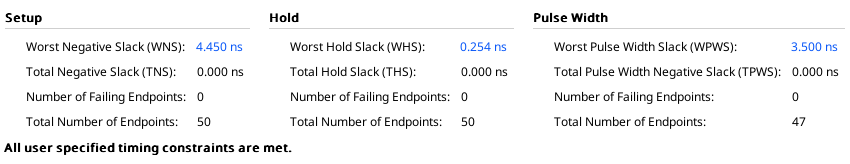
\includegraphics[width=1.0\textwidth]{../imgs/synthesis_timing_summary.png}
    
    \caption{Post-synthesis timing summary}
    \label{fig:synthesis_timing}
\end{figure}

As shown in Figure \ref{fig:synthesis_timing}, the design meets the timing requirements with a \textsl{Worst Negative Slack} of \textbf{+4.450 ns}. This means that the slowest signal arrives 4.450 ns \textbf{before} the \textsl{Required time}. In Figure \ref{fig:synthesis_critical_path} is presented this critical path:

\begin{figure}[htbp]
    \centering

    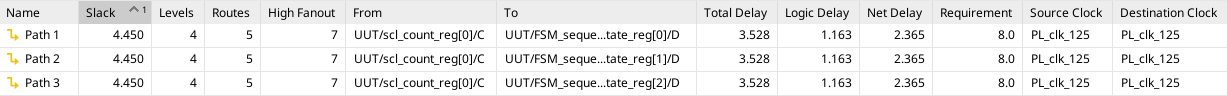
\includegraphics[width=1.0\textwidth]{../imgs/synthesis_critical_path.png}
    
    \caption{Post-synthesis critical path}
    \label{fig:synthesis_critical_path}
\end{figure}


The most critical path comes from the \texttt{scl\_count\_reg}, which is consistent with its role as the primary timing reference for the FSM. In every clock cycle the \texttt{scl\_count} is incremented, then compared to 31 and finally used to determine the next state and to update the \texttt{FSM\_sequential\_curr\_state\_reg}.

Figure \ref{fig:synthesis_timing} provided the data (\textsl{WNS}) to compute the maximum clock frequency for the Writing Master implementation. Firstly, the critical path delay ($T_{dp}$) is computed as follows:

\begin{equation}
    T_{dp} = T_{clk} - \text{WNS} = 8 \text{ ns} - 4.450 \text{ ns} = 3.55 \text{ ns}
\end{equation}

Finally, obtaining this period, the maximum clock frequency is calculated:

\begin{equation}
    F_{max} = \frac{1}{T_{dp}} = \frac{1}{3.55 \text{ ns}} \approx 281 \text{ MHz}
\end{equation}

Given these results, the clock frequency of the \IIC{} protocol, which is 32 times slower than the clock system, ranges from 3.9 MHz (at a nominal 125 MHz system clock) up to a theoretical maximum of $\approx$ 8.7 MHz ($F_{max}$). The values obtained are exceptionally high and were selected to accelerate testing and simulation analysis. As reported by \cite{wu2022basic}, the \IIC{} protocol typically operates at 100 kbps in \textit{Standard-mode}, while the fastest operational modes (such as the \textit{Ultra-Fast mode} up to 5 Mbps) omit key protocol features and operate in a write-only capacity.

\subsection{Resource utilization}

After the synthesis process, Vivado generates a report of the hardware utilization in terms of LUTs (combinational logic) and Registers (sequential logic). Table \ref{tab:synthesis_utilization} shows the post-synthesis utilization:

\begin{table}[h]
    \centering
    \label{tab:synthesis_utilization}
        \begin{tabular}{|l|c|c|c|}
        \hline
        \textbf{Resource} & \textbf{Estimation} & \textbf{Available} & \textbf{Utilization \%} \\ \hline
        LUT               & 26                  & 17600              & 0.15                    \\ \hline
        FF                & 47                  & 35200              & 0.13                    \\ \hline
    \end{tabular}
    \caption{Post-synthesis resource utilization}
\end{table}

These post-synthesis results suggest an efficient and very low hardware utilization ($< 1\%$) for both combinatorial and sequential logic. 

\subsection{Power consumption}

The post-synthesis power utilization is reported by Vivado in Figure \ref{fig:synthesis_power_consumption}:

\begin{figure}[htbp]
    \centering

    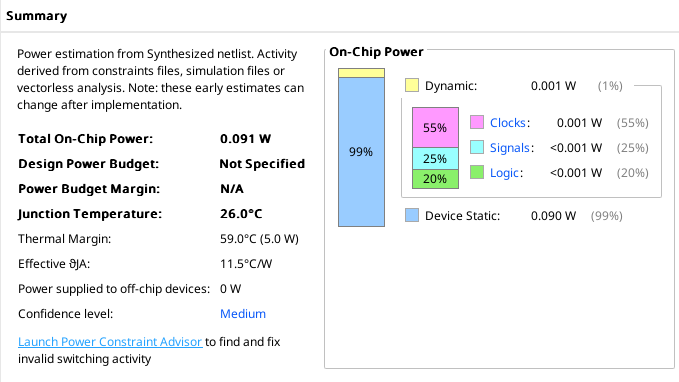
\includegraphics[width=1.0\textwidth]{../imgs/synthesis_power_consumption.png}
    
    \caption{Post-synthesis power consumption}
    \label{fig:synthesis_power_consumption}
\end{figure}

Consistent with the results of Table \ref{tab:synthesis_utilization}, 99\% of \textsl{Total On-Chip Power} is static, while the dynamic part is 1\%. This means that  most of the power is consumed to keep the device powered on, whereas a negligible part is consumed by the logic implementation.

\section{Implementation}

\subsection{Warning messages}

Before illustrating the implementation analysis, a brief comment on the warning messages encountered is reported in this section.

The implementation process terminates with success, but it reports 21 warning messages. All these warnings are caused by the \textsl{out-of-context} mode, which purposely omits all the physical I/O pin constraints. However, this doesn't affect the validity of the logic implementation.

\subsection{Timing analysis}

Similar to Section \ref{synthesis_timing}, after the implementation process terminated successfully, the \textsl{Design Timing Summary} is illustrated in Figure \ref{fig:implementation_timing_summary}:

\begin{figure}[htbp]
    \centering

    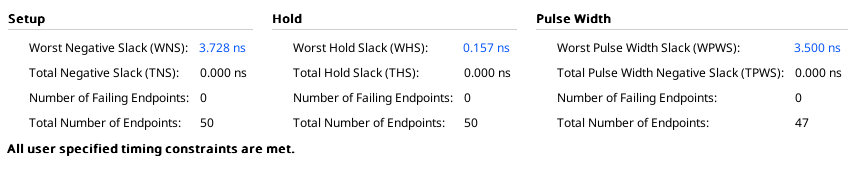
\includegraphics[width=1.0\textwidth]{../imgs/implementation_timing_summary.png}
    
    \caption{Post-implementation timing summary}
    \label{fig:implementation_timing_summary}
\end{figure}

These results validate and improve the post-synthesis timing estimation. The \textsl{Worst Negative Slack} is \textbf{+3.728 ns}, that is approximately the \textbf{6\%} less than the synthesis expectation. The critical path is approximately the same, but with different delays, as expected:

\begin{figure}[htbp]
    \centering

    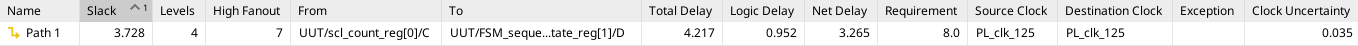
\includegraphics[width=1.0\textwidth]{../imgs/implementation_critical_path.png}
    
    \caption{Post-implementation critical path}
    \label{fig:implementation_critical_path}
\end{figure}

This decreased \textsl{WNS} indicates a lower realistic maximum frequency. In particular:

\begin{equation}
    T_{dp} = T_{clk} - \text{WNS} = 8 \text{ ns} - 3.728 \text{ ns} = 4.272 \text{ ns}
\end{equation}

\begin{equation}
    F_{max} = \frac{1}{T_{dp}} = \frac{1}{4.272 \text{ ns}} \approx 234 \text{ MHz}
\end{equation}

In conclusion, the maximum clock frequency of the \IIC{} protocol, which is 32 times slower than the clock system, will be $\approx 7$ MHz ($F_{max}$). As for the post-synthesis analysis, this value far exceeds the standard \IIC{} protocol speed.

\subsection{Resource utilization}

As for the synthesis analysis, Vivado generates a report of the hardware utilization in terms of LUTs (combinational logic) and Registers (sequential logic). Table \ref{tab:implementation_utilization} shows the post-implementation utilization:

\begin{table}[h]
    \centering
    \label{tab:implementation_utilization}
        \begin{tabular}{|l|c|c|c|}
        \hline
        \textbf{Resource} & \textbf{Estimation} & \textbf{Available} & \textbf{Utilization \%} \\ \hline
        LUT               & 26                  & 17600              & 0.15                    \\ \hline
        FF                & 47                  & 35200              & 0.13                    \\ \hline
    \end{tabular}
    \caption{Post-implementation resource utilization}
\end{table}

These results confirm the utilization obtained in the post-sytnhesis analysis.

\newpage

\subsection{Power consumption}

The post-implementation power utilization is reported by Vivado in Figure \ref{fig:implementation_power_consumption}:

\begin{figure}[htbp]
    \centering

    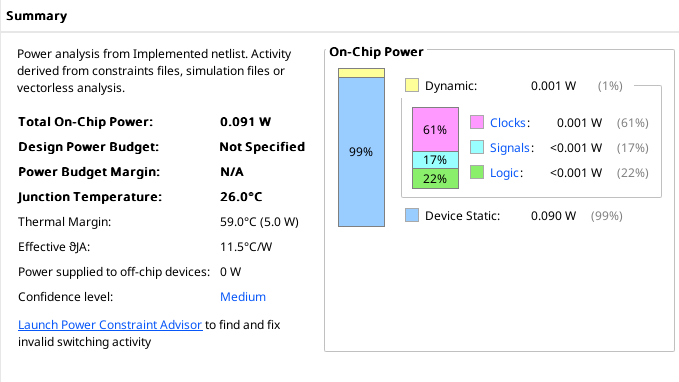
\includegraphics[width=1.0\textwidth]{../imgs/implementation_power_consumption.png}
    
    \caption{Post-implementation power consumption}
    \label{fig:implementation_power_consumption}
\end{figure}

The total dynamic power remains strictly minimal at 0.001 W, consistent with the synthesis estimates. However, the internal distribution of this dynamic power highlights the effects of the physical implementation. The power dissipated by \textsl{Signals} significantly dropped from 25\% to 17\%. This confirms the LUTs compacted placement, reducing the distance and the signal power. Consequently, the proportional weight of the \textsl{Logic} and \textsl{Clocks} slightly increased to 22\% and 61\% respectively. Overall, the total on-chip power is still dominated by the 0.090 W device static power, demonstrating the extreme power efficiency of the designed \IIC{} master module.

